\section{Deterministic local failure despite smooth convex branches}
\label{art:failure}

We now construct one objective with bad starting points at every sufficiently
small scale. The construction first realizes a contracting cycle on a maximum
of three affine functions. Carefully chosen scalar functions then place copies
of this same cycle near the unique minimizer of one fixed objective. Every
query of the implemented line search, including rejected queries, remains in
the corresponding affine region.

\subsection{The implementation and the local statement}
At a differentiable point $x$, let $g=\nabla F(x)$ and $p=-Hg$.
The line search starts with lower bracket $\ell=0$, upper bracket
$h=+\infty$, and trial length $\alpha=1$. It tests Armijo first and weak
Wolfe second:
\begin{equation}\label{art:failure_tests}
 F(x+\alpha p)\le F(x)+c_1\alpha g^Tp,
 \qquad \nabla F(x+\alpha p)^Tp\ge c_2g^Tp.
\end{equation}
An Armijo rejection sets $h=\alpha$; a Wolfe rejection sets $\ell=\alpha$.
The next length is $(\ell+h)/2$ when $h<\infty$, and $2\ell$ otherwise.
If both tests hold, the length is accepted. This is the unit-first
bracketing implementation of Lewis--Overton~\cite[Algorithm~4.6]{LO}.
All comparisons in the construction are strict, so strict acceptance tests
give the same decisions.

Write the full inverse update as
\begin{equation}\label{art:failure_update}
 \mathcal B(H,g,g^+,\alpha)
 =\left(I-\frac{sy^T}{y^Ts}\right)H
  \left(I-\frac{ys^T}{y^Ts}\right)+\frac{ss^T}{y^Ts},
 \quad s=-\alpha Hg,\quad y=g^+-g.
\end{equation}
No resetting or rescaling of the stored matrix is performed.

The local counterexample is Theorem~\ref{art:local-failure}; we prove it below.

The theorem concerns a specified implementation and a sequence of starting
points. It does not assert failure for every nearby start or a positive-measure
basin. Its branches have no uniform positive lower curvature bound.
The construction differs from the nonconvex prescribed-orbit examples
of Mascarenhas~\cite{NEG_M04,NEG_M07}: here convexity, the unique nearby
minimizer, fixed identity initialization and all-query containment are
proved simultaneously.

\subsection{A finite cycle controlling the entire trial tree}
Let $(c,d)$ be the algebraic pair specified in
Appendix~\ref{art:seed_certificate}. Define
\[
 g_0=(1,0)^T,\qquad g_1=(-1,-1/8)^T,\qquad g_2=(c,d)^T,
 \qquad G(z)=\max_{0\le i\le2}g_i^Tz.
\]
The useful coarse bounds are $0.318<c<0.319$ and
$-1.026<d<-1.025$. Put
\begin{equation}\label{art:seed_rho}
 \rho=\frac{129(c-8d)}{(16c-127d-16)(127c+16d+129)},
 \qquad 0.060<\rho<0.061.
\end{equation}
Set
\begin{align}
 M_0&=I,\quad
 M_1=\begin{pmatrix}129/256&-1/16\\-1/16&1\end{pmatrix},
 &M_2&=\mathcal B(M_1,g_1,g_2,1/4),\label{art:seed_matrices}\\
 s_0&=(-1,0)^T,\quad s_1=(127/1024,1/64)^T,
 &s_2&=\rho(1-c,-d)^T.\label{art:seed_steps}
\end{align}
Finally, let
\begin{equation}\label{art:seed_points}
 z_0=\frac1{1-\rho}
 \begin{pmatrix}897/1024-\rho(1-c)\\ \rho d-1/64\end{pmatrix},
 \qquad z_{j+1}=z_j+s_j\quad(j=0,1,2).
\end{equation}

\begin{lemma}[Exact cycle and strict trial decisions]\label{art:seed_cycle}
The matrices in \eqref{art:seed_matrices} are positive definite, and
\[
 \mathcal B(I,g_0,g_1,1)=M_1,\qquad
 \mathcal B(M_2,g_2,g_0,1/16)=\rho I,\qquad z_3=\rho z_0.
\]
At $z_j$, $j=0,1,2$, the unique active gradient is $g_j$.
With $p_j=-M_jg_j$, the entire line-search query list is
Table~\ref{art:trial_table}. At every rejection the objective strictly
exceeds its current value. At every acceptance,
\begin{equation}\label{art:seed_margins}
 G(z_j)+\tfrac13g_j^Ts_j-G(z_{j+1})>0,\qquad
 g_{j+1}^Ts_j>0>g_j^Ts_j,
\end{equation}
where $g_3=g_0$. All listed queries and the three starting points have a
unique active branch and satisfy
\begin{equation}\label{art:seed_query_bounds}
 |g_i^Tz|<3 (i=0,1,2),\qquad z_2<2,\qquad G(z)>0.
\end{equation}
Here $z_2$ in the middle inequality denotes the second coordinate.
\end{lemma}

\begin{table}[t]
\centering
\begin{tabular}{ccccc}
\hline
Phase $j$ & Trial $\alpha$ & Active branch & $10^4G(z_j+\alpha p_j)$ & Decision\\
\hline
0&1&1&$(1218,1219)$&accept\\
1&1&0&$(3845,3846)$&reject\\
1&$1/2$&0&$(1364,1365)$&reject\\
1&$1/4$&2&$(723,724)$&accept\\
2&1&0&$(6687,6691)$&reject\\
2&$1/2$&0&$(3406,3408)$&reject\\
2&$1/4$&0&$(1765,1767)$&reject\\
2&$1/8$&0&$(944,946)$&reject\\
2&$1/16$&0&$(534,536)$&accept\\
\hline
\end{tabular}
\caption{Rational enclosures and the deterministic trial tree for the
algebraic seed. Every rejection is an Armijo rejection. The intervals are
enclosures, not rounded approximations asserted to be exact values.}
\label{art:trial_table}
\end{table}

The proof of the lemma, including the rational certificate and its soundness,
is in Appendix~\ref{art:seed_certificate}. It implies the decisions for all
parameters in Theorem~\ref{art:local-failure}: an accepted decrease is
greater than one third of its predicted decrease, and its new directional
derivative is positive. No Wolfe rejection is needed, so the query lengths
are exactly the successive bisections displayed in the table.

Figure~\ref{art:cycle-figure} displays this unit-first geometry: phase zero
accepts its first query, while the next two phases bisect past the rejected
candidates before reaching their accepted points. The right panel includes
all those rejected candidates.

\begin{figure}[t]
\centering
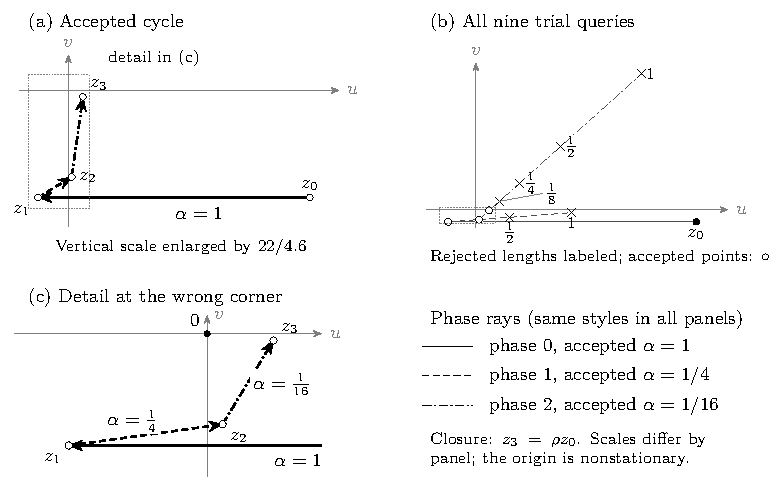
\includegraphics[width=\textwidth]{figures/cycle_trials.pdf}
\caption{The accepted three-step seed cycle (left), with closure
$z_3=\rho z_0$, and every rejected candidate point (right). The rendering
uses the rational center of the certified root box. It illustrates the
certified trial geometry; it is not a proof of exact equality or of
membership in the stable manifold used for the perturbed construction.}
\label{art:cycle-figure}
\end{figure}

Homogeneity and the two cycle closures now give an infinite induction:
\begin{equation}\label{art:cone_orbit}
 x_{3m+j}=\rho^mz_j,\qquad H_{3m+j}=\rho^mM_j,\qquad j=0,1,2.
\end{equation}
Each query in phase $j$ is $\rho^m$ times its base query. Gradients are
unchanged, function differences and gradient--step products scale by
$\rho^m$, and \eqref{art:failure_update} scales the updated matrix by
$\rho^m$. Thus every branch choice and every rejection is preserved, as
well as acceptance. The iterates converge to zero, but the direction
$w=(-1,16)^T$ satisfies
\[
 g_0^Tw=g_1^Tw=-1,\qquad g_2^Tw=-c+16d<-1.
\]
Hence $G(tw)=-t$ for $t\ge0$, so this limit is nonstationary.

\begin{corollary}[Coercive polyhedral global failure]\label{art:failure_polyhedral}
The same deterministic run, with $H_0=I$, fails for
\[
 \overline G(u,v)=\max\{u,-u-v/8,cu+dv,v-17\}.
\]
This function is coercive and has unique minimizer $(-1,16)$, with value
$-1$, while the run converges to the nonstationary origin with value zero.
\end{corollary}
\begin{proof}
At every query, \eqref{art:seed_query_bounds} and $0<\rho<1$ give
$v-17<0<G(u,v)$, so the fourth branch is inactive. The convex combination
of branches $0,1,3$ with weights $8/17,8/17,1/17$ is identically $-1$.
Equality in this lower bound forces all three branches to equal $-1$,
hence $(u,v)=(-1,16)$; the remaining branch is strictly smaller there.
If $\overline G(u,v)\le t$, then
$u\le t$, $v\le t+17$ and $-u-v/8\le t$, which also give lower bounds
on both coordinates. Every sublevel is therefore compact.
\end{proof}
This corollary concerns global failure at a wrong corner. The next step
places such corners arbitrarily near the true minimizer of one objective.

\subsection{Scalar interpolation with affine regions at every scale}
Let $\theta=1/16$, $a_n=\theta^n$, $\varepsilon=1/128$, and
$b_*=2c-32d\in(33,34)$. For $b\in\{2,b_*\}$ define
\[
 t_b=\frac{1-(1+\theta+\theta^2)/b}{1-\theta^2},\qquad
 v=\frac{\xi-t_b+\varepsilon}{2\varepsilon}.
\]
\[
 P_b(\xi)=
 \begin{cases}
 0&\xi\le t_b-\varepsilon,\\
 3v^2-2v^3&|\xi-t_b|<\varepsilon,\\
 1&\xi\ge t_b+\varepsilon,
 \end{cases}
 \quad J_b(\xi)=\int_0^\xi P_b(t)\,dt.
\]
The middle formula for $J_b$ is $2\varepsilon(v^3-v^4/2)$; its outer
formulas are zero and $\xi-t_b$. For
$b\theta a_n\le x\le ba_n$, set
\begin{equation}\label{art:upper_scalar}
 \varphi_b(x)=(\theta a_n)^3+
 ba_n^3(1-\theta)
 \{\theta^2\xi+(1-\theta^2)J_b(\xi)\},\qquad
 \xi=\frac{x/(ba_n)-\theta}{1-\theta}.
\end{equation}
Complete the definition by
\[
 \varphi_b(x)=
 \begin{cases}
 1-3(x+1)+3(x+1)^2&x<-1,\\
 -x^3&-1\le x\le0,\\
 1+x-b&x\ge b.
 \end{cases}
\]

\begin{lemma}[Scalar interpolation]\label{art:upper_scalar_lemma}
The functions $\varphi_b$ are convex, coercive and globally $C^{2,1}$,
are nonnegative, and vanish only at zero. They satisfy
\begin{align}
 0&\le\varphi_b''\le\max\{6,102/b\},\label{art:scalar_curvature}\\
 \varphi_b(ba_n+h)&=a_n^3+a_n^2h
       \qquad(|h|\le a_n/2).\label{art:scalar_plateau}
\end{align}
Their second derivatives are globally Lipschitz with constant
\[
 L_b=\max\{6,139264/(5b^2)\}.
\]
\end{lemma}
\begin{proof}
The ramp is monotone, $C^1$, and satisfies
$0\le P_b'\le96$ and $\int_0^1P_b=1-t_b$. On a positive interval,
\[
 \varphi_b'=a_n^2\{\theta^2+(1-\theta^2)P_b(\xi)\},\qquad
 \varphi_b''=\frac{a_n(1+\theta)}bP_b'(\xi).
\]
The identity
$\theta^2+(1-\theta^2)(1-t_b)=(1+\theta+\theta^2)/b$
gives matching values $\varphi_b(ba_n)=a_n^3$. The derivative is
constant near both ends of each interval, so the first two derivatives
also match, with values $a_n^2$ and zero at $ba_n$.

As $x\downarrow0$, the bounds $a_n\le x/(b\theta)$ on its interval
give $\varphi_b(x)=O(x^3)$, $\varphi_b'(x)=O(x^2)$ and
$\varphi_b''(x)=O(x)$. These match the negative cubic at zero.
The formulas also match through second order at $-1$ and $b$.
The derivative is negative on the negative half-line and positive on the
positive half-line; the outer formulas diverge to infinity. This proves
convexity, coercivity and the minimum assertions.

The constant-derivative lengths below and above $ba_n$, divided by $a_n$,
are
\[
 b(1-\theta)(1-t_b-\varepsilon),\qquad
 \frac{b(1-\theta)(t_b-\varepsilon)}\theta.
\]
Both exceed $1/2$ for $2\le b\le34$, by substitution in the displayed
rational formulas; the affine outer extension covers the upper side when
$n=0$. This proves \eqref{art:scalar_plateau}.
Finally $|P_b''|\le3/(2\varepsilon^2)$ in each ramp, so differentiation
once more gives $|\varphi_b'''|\le139264/(5b^2)$ there. The negative
cubic has third derivative of magnitude six. Continuity of
$\varphi_b''$ permits summing the Lipschitz estimates over finitely many
joins away from zero; taking limits at zero covers the infinitely many
accumulating joins and gives the global bound.
\end{proof}

\subsection{One objective and a uniform induction over all queries}
Define
\begin{equation}\label{art:upper_objective}
 F(u,v)=\max\{\varphi_2(u),\varphi_2(-u-v/8),
                    \varphi_{b_*}(cu+dv),v\}.
\end{equation}
The Hessian of each of the first three branches is a nonnegative scalar
multiple of $g_ig_i^T$. Equation~\eqref{art:scalar_curvature} gives the
upper bounds $51$, $51(65/64)<52$, and $12$, respectively, on their
operator norms; the last branch has zero Hessian. Their Hessians are
globally Lipschitz because $\varphi_b''$ is Lipschitz and the arguments
are linear. The first two scalar arguments are independent, so their
coercivity makes every sublevel of $F$ compact. Nonnegativity and their
unique scalar zeros show $F(x)=0$ exactly at $x=0$. At zero the first
three gradients vanish and the last is $(0,1)^T$, giving
$F'(0;h)=\max\{0,h_2\}$; thus the minimizer is nonsmooth.

Let $p_n=a_n(2,-32)^T$. The first two scalar arguments at $p_n$ equal
$2a_n$, and the third equals $b_*a_n$. Consequently
\begin{equation}\label{art:upper_local_model}
 F(p_n+h)=a_n^3+a_n^2G(h)
 \quad\hbox{if } |g_i^Th|\le a_n/2 (i=0,1,2).
\end{equation}
Indeed, the first three branches are on their affine regions and each
has value at least $a_n^3/2$. The first two slab inequalities imply
$|h_1|\le a_n/2$ and $|h_2|\le8a_n$, so the fourth branch is negative.
In particular $F(p_n)=a_n^3$ and
$F'(p_n;(-1,16)^T)=-a_n^2<0$.

\begin{proof}[Proof of Theorem~\ref{art:local-failure}]
For $n\ge1$ take $x_0^{(n)}=p_n+a_n^2z_0$ and $H_0=I$. We claim that
\begin{equation}\label{art:upper_orbit}
 x_{3m+j}^{(n)}=p_n+a_n^2\rho^mz_j,\qquad
 H_{3m+j}^{(n)}=\rho^mM_j,\qquad j=0,1,2.
\end{equation}
At a current point of this form its gradient is $a_n^2g_j$. Every trial
on the finite candidate list therefore has the form
$p_n+a_n^2\rho^mz_{\rm trial}$. Equation~\eqref{art:seed_query_bounds}
gives
\[
 |g_i^T(a_n^2\rho^mz_{\rm trial})|<3a_n^2
 \le3a_n/16<a_n/2.
\]
Thus \eqref{art:upper_local_model} is valid at every candidate query,
not only the final accepted one. Unique activity is preserved, and
\[
 F(p_n+a_n^2\rho^mz_{\rm trial})
   =a_n^3+a_n^4\rho^mG(z_{\rm trial}),\qquad
 \nabla F=a_n^2g_{\rm active}.
\]
The additive constant cancels in Armijo. Function differences and
gradient--step products are the seed quantities multiplied by the same
positive factor $a_n^4\rho^m$. The actual search therefore traverses
exactly the candidate list and makes the same strict decisions.
In \eqref{art:failure_update}, the projection factors are unchanged and
the rank-one term has factor $\rho^m$. The cycle closures prove the next
point and matrix identities, completing the induction.

The finite matrices are positive definite. Equation~\eqref{art:upper_orbit}
gives convergence to $p_n$ and strict descent to $a_n^3>0$.
Since the base query set is finite, the norm of every query is bounded by
\[
 a_n\|(2,-32)\|+a_n^2\max_{\text{base points and queries}}\|z\|,
\]
which tends to zero. The starting points also tend to zero. All other
claims were proved directly from \eqref{art:upper_objective}.
\end{proof}
